\section{Factor-Contrastive Sparse Autoencoder}
\label{sec:method}

The method uses observed relations to determine how a sparse dictionary should organize its features. A relation sampler first states what each route should treat as equivalent and what it must distinguish. A blockwise sparse autoencoder then learns these relations while reconstructing the original activation. Figure~\ref{fig:factor-sae-method} summarizes this two-stage design.

\subsection{Controlled relations define route semantics}

Let $H(x)\in\mathbb{R}^{d}$ be the frozen pooled activation of utterance $x$. Each utterance has an intent $C$ and a locale $S$. The intent route $z_C$ should respond similarly when intent is fixed and locale changes. The locale route $z_S$ should exhibit the reciprocal behavior.

The key comparison is easiest to see from one anchor $x_a$ with intent $c_a$ and locale $s_a$. For $z_C$, the positive keeps the anchor intent but changes locale. The opposing example keeps the anchor locale but changes intent. Formally,
\begin{equation}
\begin{aligned}
C(x_C^+)&=c_a, & S(x_C^+)&\neq s_a,\\
C(x_C^-)&\neq c_a, & S(x_C^-)&=s_a.
\end{aligned}
\label{eq:c-relations}
\end{equation}
This pairing makes the desired distinction explicit: the positive changes the nuisance factor, whereas the opposing example matches it. The $z_S$ route reverses the same pair, using $x_S^+=x_C^-$ and $x_S^-=x_C^+$. It therefore preserves locale while opposing intent.

On MASSIVE, half of the $z_C$ positives are exact translations and half are different semantic IDs with the same intent. Every opposing example has a different intent and the anchor locale. The 50/50 mixture prevents the intent relation from reducing to sentence identity; sampling is balanced over the complete relation set.

\begin{proposition}
If negatives for $z_C$ are matched on $S$, a representation that depends only on $S$ cannot rank $x_C^+$ above $x_C^-$ for every relation.
\label{prop:matched-shortcut}
\end{proposition}
An $S$-only representation maps $x_a$ and $x_C^-$ to the same value, making the opposing similarity maximal, while $x_C^+$ changes $S$. It therefore cannot satisfy every $z_C$ relation. Appendix~\ref{app:shortcut-proof} gives the formal argument; the reciprocal construction gives the same protection to $z_S$.

\subsection{Learning the relations in a sparse dictionary}

The relations supervise sparse features directly rather than first creating a dense bottleneck. A shared encoder maps $H(x)$ into one overcomplete pre-activation vector and assigns disjoint coordinates to the two routes:
\begin{equation}
\begin{aligned}
a(x)&=W_{\mathrm{enc}}H(x)+b_{\mathrm{enc}},\\
a&=[a_C;a_S]\in\mathbb{R}^{m}.
\end{aligned}
\end{equation}
A single global sparsity budget could allow one route to consume nearly all active features. We instead apply BatchTopK separately to the two blocks \citep{bussmann2024batchtopk}:
\begin{equation}
\begin{aligned}
z_C&=\operatorname{BatchTopK}_{k_C}(a_C),\\
z_S&=\operatorname{BatchTopK}_{k_S}(a_S).
\end{aligned}
\label{eq:sparse-routes}
\end{equation}
For a batch of $B$ examples, the blocks retain their largest $Bk_C$ and $Bk_S$ positive activations. Each example may use more or fewer features, but each route receives a guaranteed mean activity budget. Training-calibrated thresholds make test-time inference independent of batch composition.

The exact blockwise control uses the same encoder, route widths, activity budgets, decoder, and optimizer but removes both relational losses. Its difference from the proposed model therefore isolates the effect of controlled relations rather than the block allocation.

The decoder reconstructs the original activation from the concatenated code:
\begin{equation}
\widehat H=W_{\mathrm{dec}}[z_C;z_S]+b_{\mathrm{dec}},\qquad
\mathcal{L}_{\mathrm{rec}}=\lVert H-\widehat H\rVert_2^2.
\label{eq:reconstruction}
\end{equation}
Following standard Top-$k$ SAE training \citep{gao2024scaling}, decoder columns are normalized after every optimization step.

\begin{figure*}[t]
\centering
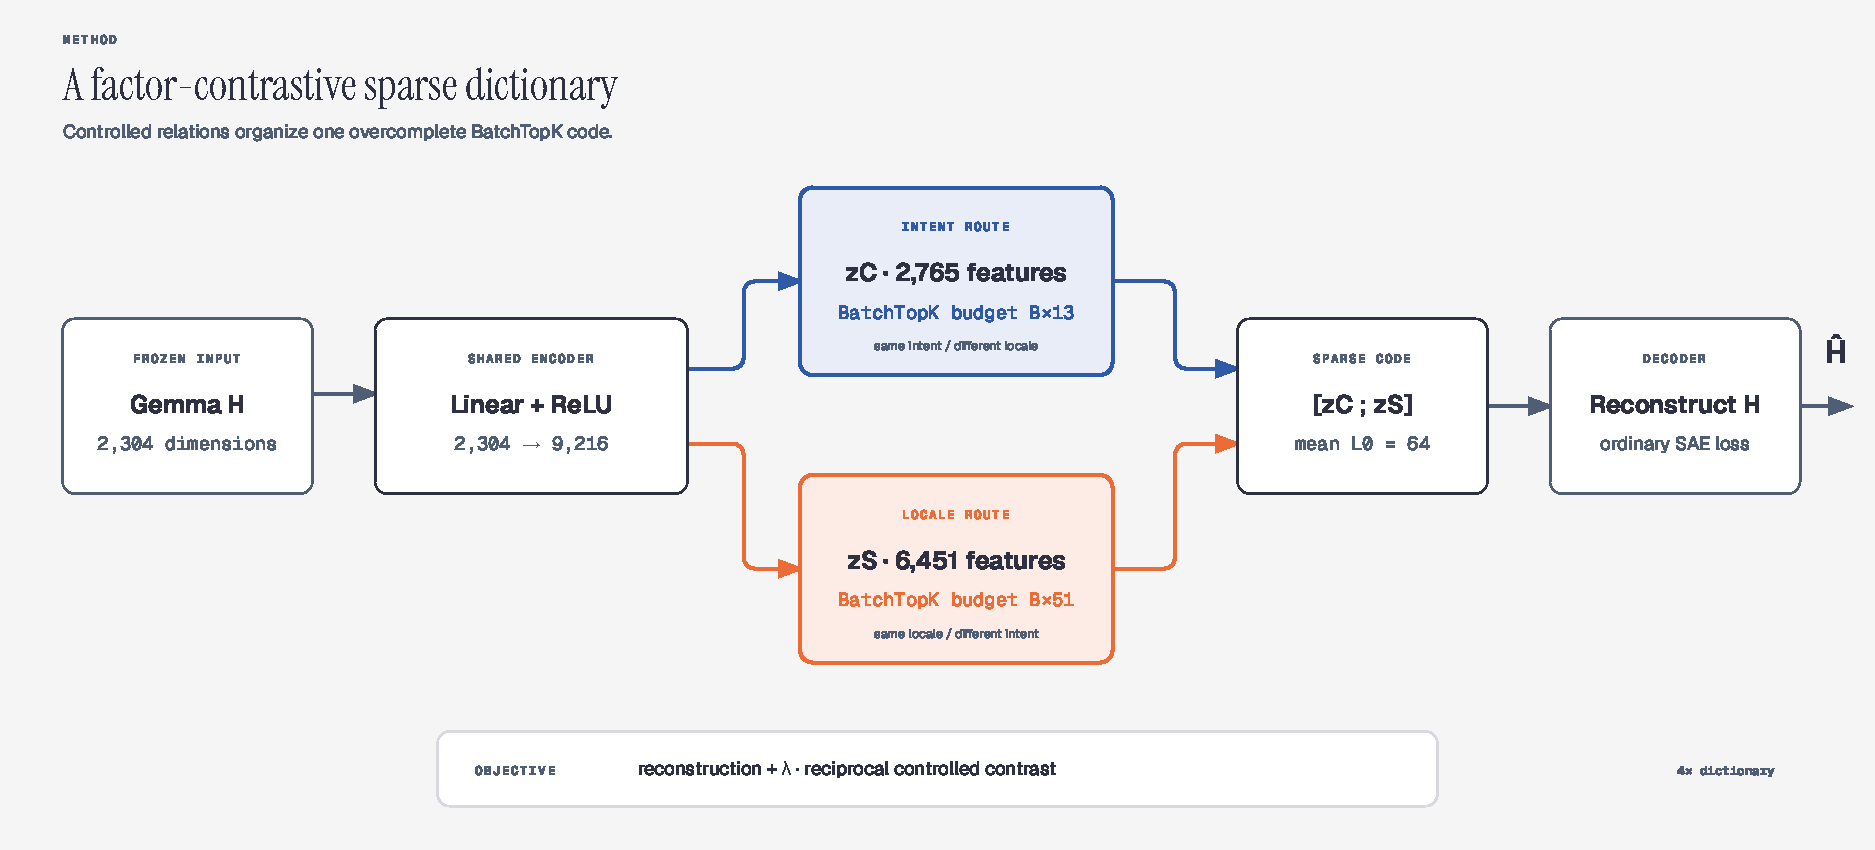
\includegraphics[width=\textwidth]{Figures/factor_sae_figure1_method.pdf}
\caption{Factor-contrastive sparse autoencoder. A shared encoder maps frozen activations into one overcomplete dictionary. Blockwise BatchTopK assigns separate activity budgets to the intent- and locale-dominant routes; reciprocal controlled relations organize the routes while an ordinary linear decoder reconstructs the input activation.}
\label{fig:factor-sae-method}
\end{figure*}

The relational objective asks each route to rank its positive above its matched opposing example. For route $r\in\{C,S\}$, let $\bar z_r=z_r/\lVert z_r\rVert_2$, $u_r^+=\bar z_r(x_a)^\top\bar z_r(x_r^+)$, and $u_r^-=\bar z_r(x_a)^\top\bar z_r(x_r^-)$. We use the standard contrastive softmax form \citep{oord2018cpc,zimmermann2021contrastive}:
\begin{equation}
\begin{aligned}
\mathcal{L}_r&=-\log\frac{\exp(u_r^+/\tau)}
{\exp(u_r^+/\tau)+\exp(u_r^-/\tau)},\\
\mathcal{L}&=\mathcal{L}_{\mathrm{rec}}
+\frac{\lambda}{2}(\mathcal{L}_C+\mathcal{L}_S).
\end{aligned}
\label{eq:route-loss}
\end{equation}
The first term preserves ordinary SAE reconstruction; the two relational terms determine which factor organizes each route. No adversarial, orthogonality, independence, prototype, or swap-training term is used.

The main model uses a fourfold dictionary; an eightfold version tests sparse-width sensitivity. Appendix~\ref{app:protocol} gives the exact route dimensions and activity budgets. Complementarity is evaluated from the learned routes rather than imposed by an auxiliary constraint.
